% Das Management Summary richtet sich in der Praxis an die "Chefs des Chefs", d.
% h. an die Vorgesetzten des Auftraggebers (diese sind in der Regel keine
% Fachspezialisten).
% Die Sprache soll knapp, klar und stark untergliedert sein.
% Zu verwenden ist folgenden Gliederung:
% - Ausgangslage - Vorgehen, Technologien - Ergebnisse - Ausblick (optional)

\chapter*{Management Summary}\addcontentsline{toc}{chapter}{Management Summary}

\paragraph{Ausgangslage}~\\
Die heute gängigen \glspl{Routing-Engine} können effizient über Knoten und Kanten routen und wurden konkret für den motorisierten Individualverkehr optimiert. Für den nicht-motorisierten Individualverkehr (Fussgänger, Rollstuhlfahrer, Radfahrer, etc.) sieht die Lage drastisch anders aus. Der motorisierte Individualverkehr hält sich durchwegs an vorgegebene Regeln und Strecken. Ein Fussgänger hingegen verhält sich grundlegend auf eine andere Art und Weise. Wo ein Autofahrer an die Streckenführung gebunden ist, optimiert ein Fussgänger intuitiv. So überquert er einen Platz auf direktem Weg und läuft nicht an der Strasse um den Platz herum, wie es ein Autofahrer tun muss. Dies ist in den Routing-Engines jedoch Status quo. In Abbildung \ref{fig:compare_fischmarktplatz} ist sichtbar, wie über den Fischmarktplatz in Rapperswil-Jona, Schweiz geroutet wird. Es liegt in der Natur des Menschen, den Platz ressourcenschonend zu überqueren, was momentan nicht der Fall ist.

Die Problematik beschränkt sich nicht nur auf Flächen wie Plätze und Parks, sondern umfasst auch Strassen und weitere Arten von offenen Flächen wie Berge und Strände.

Durch den Einzug der mobilen Geräte ist es üblich, dass von einem beliebigen Startpunkt aus das Routing gestartet wird. Befindet man sich in diesem Fall gerade auf einer Fläche, wird aktuell eine Mittelsenkrechte zur Kante gezogen, auf welcher das Routing fortgesetzt wird.

Ein Fussgänger ist in vielen Fällen auf die öffentlichen Verkehrsmittel angewiesen, was in einem multimodalen Routing resultiert. Das genaue Ansteuern einer bestimmten ÖV-Haltestelle in die richtige Fahrtrichtung gestaltet sich schwierig, da für eine ÖV-Haltestelle die gleiche Koordinate für beide Fahrtrichtungen von verschiedenen Services retourniert wird. Für ein Fussgänger-Routing ist dies suboptimal, da sich diese Koordinate in manchen Fällen direkt auf einer Haupstrasse befinden kann und ÖV-Haltestellen nicht immer auf der gegenüberliegenden Strassenseite liegen müssen.

\begin{figure}[ht]
    \centering
    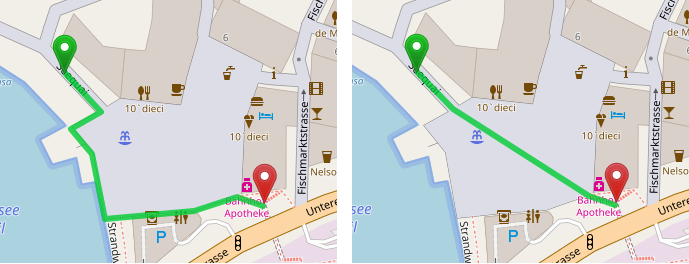
\includegraphics[width=1\linewidth]{technicalreport/img/compare_fischmarktplatz.png}
    \caption[Vergleich Ausgangslage und Ergebnis]{Vergleich aktueller Stand einer Routing-Engine (links) mit dem Ergebnis der Vorverarbeitung (rechts); Fischmarktplatz in Rapperswil-Jona, Schweiz; Screenshot aufgenommen am 17.12.17}
    \label{fig:compare_fischmarktplatz}
\end{figure}


\paragraph{Ziele, Vorgehen und Technologien}~\\
Im Kontext der Arbeit \emph{PlazaRoute} wird die Problematik des Fussgänger-Routings über offene Flächen im urbanen Raum aufgegriffen. Kurz zusammengefasst heisst das, dass eine \gls{Routing-Engine} ein natürliches Fussgänger-Routing generieren kann.

In Kombination mit dem ÖV-Routing soll ein multimodales Routing möglich sein, welches von einem beliebigen Startpunkt aus an eine Zieldestination routet und dabei ÖV-Haltestellen genau ansteuert.

Um diese Anforderungen erfüllen zu können, werden Algorithmen zum Traversieren von offenen Fussgänger-Flächen evaluiert, analysiert, getestet und optimiert. Nach Abschluss dieser Tätigkeit wird es möglich sein, eine \ac{OSM} Datei so aufbereiten zu können, dass \glspl{Routing-Engine} dem Fussgänger ein natürliches Routing bieten können. Die durch die Algorithmen erzeugten Graphen werden mit \gls{Shortest-Path}-Algorithmen vereinfacht, um die zusätzliche Datenmenge zu minimieren.

Um die Optimierung an einem praktischen Beispiel zeigen zu können, wird parallel in Kombination mit dem Service von search.ch ein Backend für ein multimodales Routing entwickelt. Dies wird durch eine visuelle Darstellung in einem \gls{QGIS}-Plugin abgerundet, welche den Mehrwert für einen Fussgänger konkret aufzeigen wird.

Die zugrundeliegende Technologie ist Python.

\paragraph{Ergebnisse}~\\
Durch die Umsetzung einer Vorverarbeitung mit einem Visibility-Graph oder SpiderWeb-Graph in Kombination mit einem \gls{Shortest-Path}-Algorithmus (Dijkstra oder A*) ist die Grundlage für ein natürliches Fussgänger-Routing geschaffen, auf welcher gängige Routing-Engines und andere Interessenten operieren oder auf der Implementation aufsetzen können.

Fussgänger können zu jedem Zeitpunkt und von jeder Position aus ein Routing durchführen, welches ihrem Verhalten entspricht.

\begin{figure}[H]
    \centering
    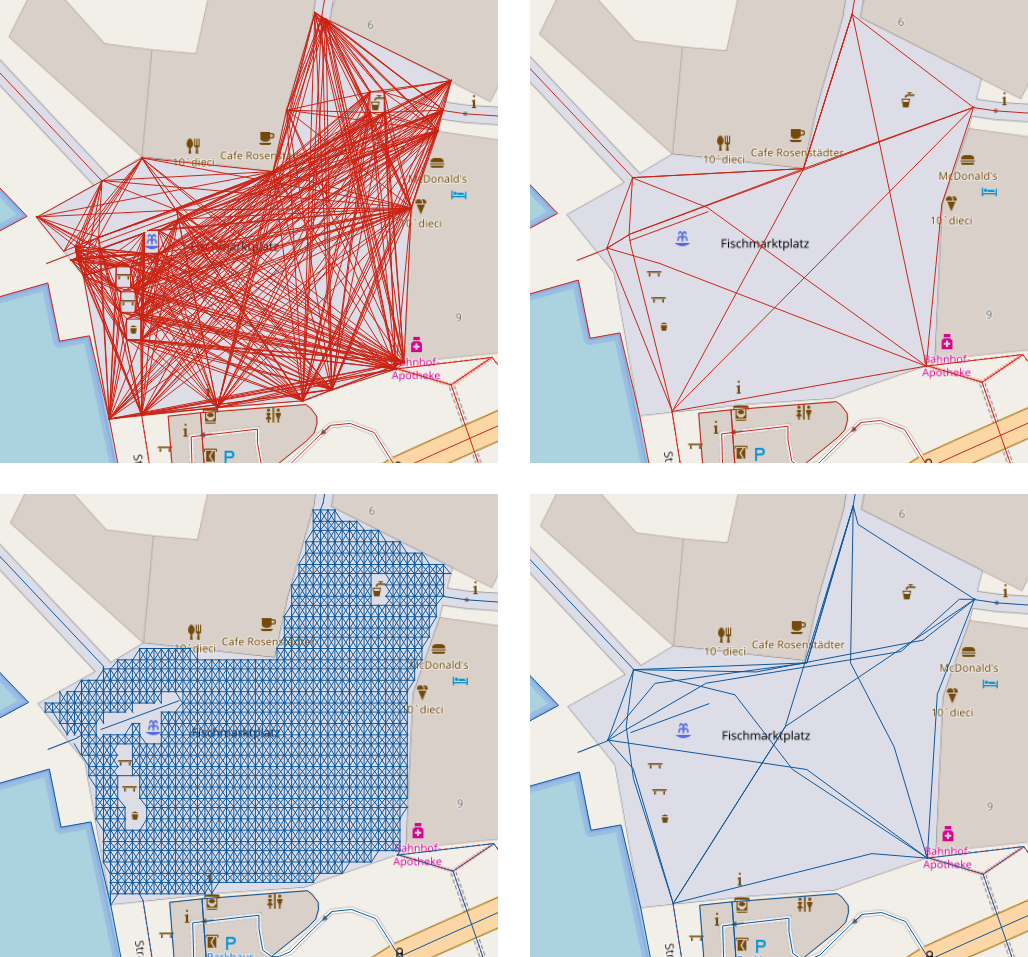
\includegraphics[width=0.8\linewidth]{technicalreport/img/proprecessing_optimization_comparison.png}
    \caption[Vergleich Preprocessing mit und ohne Optimierung]{Vergleich der Algorithmen Visibility-Graph (oben) und SpiderWeb-Graph (unten), vor und nach der Optimierung durch \gls{Shortest-Path}-Algorithmen}
    \label{fig:proprecessing_optimization_comparison}
\end{figure}

Um bequem und auf direktem Weg nach Hause zu gelangen, ist das transportmittelübergreifende Routing als Service verfügbar und kann in einem QGIS-Plugin visualisiert werden.

\begin{figure}[H]
    \centering
    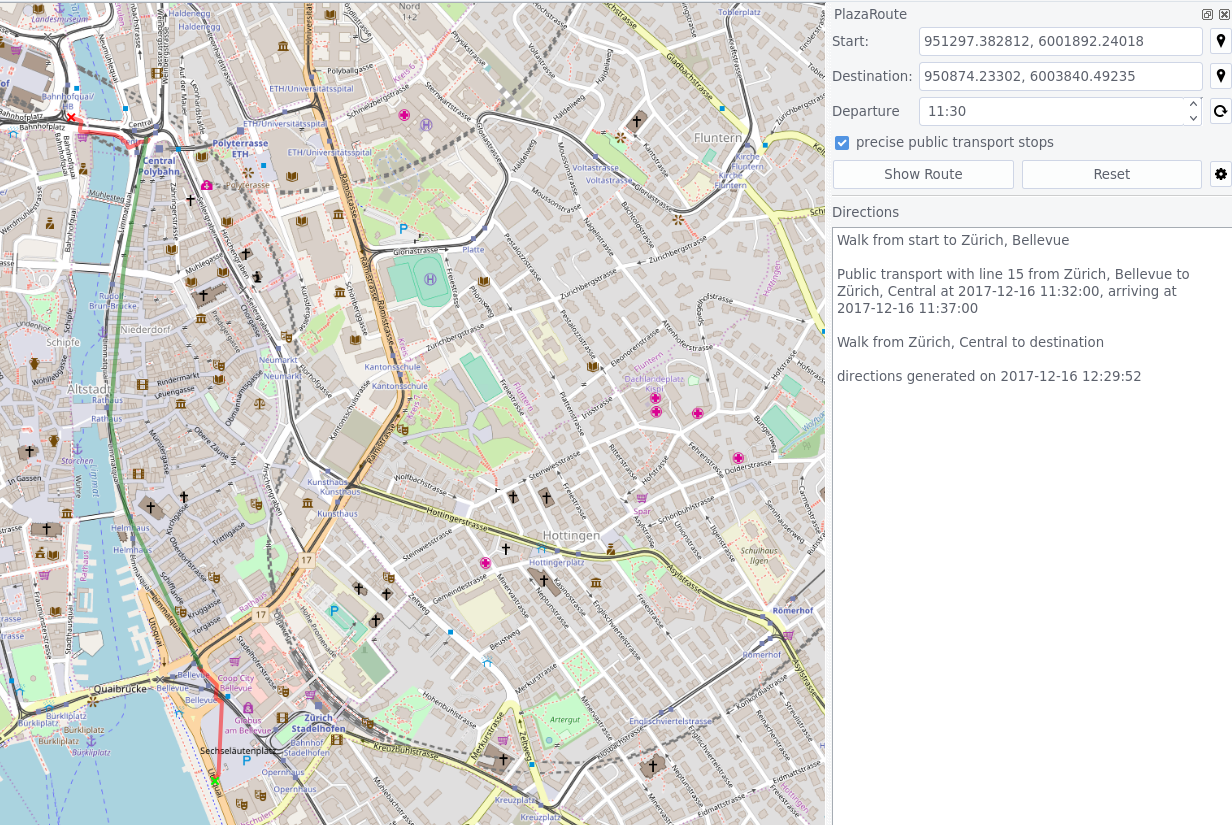
\includegraphics[width=1.0\linewidth]{technicalreport/img/qgis_plugin_plaza_route_cropped}
    \caption[Berechnete Route in QGIS-Plugin PlazaRoute]{Berechnete Route in QGIS-Plugin PlazaRoute}
    \label{fig:qgis_plugin_plaza_route_cropped}
\end{figure}

\paragraph{Ausblick}~\\
Die bestehende Lösung bietet weiteren Raum für Optimierungen. So können einige Flächen, welche für Fussgänger begehbar sind, durch fehlende \glspl{Einstiegspunkt} momentan nicht verarbeitet werden.

Die Arbeit hat sich bewusst auf den urbanen Raum beschränkt, da die Mehrheit der Routings in diesem Umfeld durchgeführt werden. Diese Grenze soll erweitert werden und Flächen ohne konkrete Begrenzungen wie Berge und Strände einbeziehen.

Die Vorverarbeitungen der Flächen stösst im Bezug auf die Performanz an Grenzen. Ein Vergleich mit einer Lösung in PostGIS oder C++ ist denkbar.